% !TeX spellcheck = en_US

\documentclass[a4paper,12pt]{article}

\usepackage{alltt, fancyvrb, url}
\usepackage{graphicx}
\usepackage{subfigure}
\usepackage{wrapfig}
\usepackage{algorithmic}
\usepackage[utf8]{inputenc}
\usepackage{fontenc}
\usepackage{amsmath,stmaryrd,mathtools,algorithm}
\usepackage{amssymb}
\usepackage{longtable}
\usepackage{multirow}
\usepackage{setspace}
\usepackage{listings}
\usepackage{todonotes}
\usepackage{csquotes}
\usepackage[margin=1.0in]{geometry}

% Remove option to use English naming
\usepackage[colorlinks,
linkcolor={red!70!black},
citecolor={blue!80!black},
urlcolor={blue!50!black}]{hyperref}
\usepackage[nameinlink]{cleveref}

\title{}
\setcounter{tocdepth}{3}
\setcounter{secnumdepth}{3}

\author{Dario Pavllo -- dario.pavllo@epfl.ch}
\date{} %\today

\begin{document}
\pagenumbering{gobble}
%\maketitle
{
\centering
\subsection*{Decentralized systems engineering -- Final report\\``Secure and anonymous private messaging''\\Dario Pavllo -- \texttt{dario.pavllo@epfl.ch}}}

\section{Introduction} % 2 sentences
The goal of this project is to build a robust, scalable messaging system that provides end-to-end encryption (as Telegram or Whatsapp do) in a decentralized manner, and that guarantees anonymity as well as authentication (i.e. signed messages) by using public-key cryptography. This topic is relevant because people are putting less trust into governments and are willing to take extra precautions in order to improve their privacy; additionally, this project poses some interesting technical challenges and trade-offs that are worth exploring.

\section{Goals and functionalities} % 0.75 pages
The basic idea is to have a messaging system where messages are stored on the network and can be retrieved by the parties at any time. Messages are exchanged through a gossip mechanism that resembles the first version of Peerster, but with an additional security layer. The main features of the project can be summarized as follows:
\begin{itemize}
	\item \textbf{Public and private messaging:} users can send messages to a public chat room, as well as private messages to other users.
	\item \textbf{Anonymous and decentralized name infrastructure:} this point borrows some ideas from Tor and Bitcoin. There is no actual name registration procedure for using the system. Instead, users generate a public/private key pair (this can be done on-the-fly) and are uniquely identified by their public key. The public key is then used to derive a unique username, just like Bitcoin wallets or Tor hidden services (e.g. \texttt{blockchainbdgpzk.onion}). These names are said to be \emph{self-authenticating} because they can be easily verified and cannot be forged. This approach does not rely on a name service (which requires consensus in order to avoid conflicts), and can therefore scale well in a decentralized scenario. Moreover, it is intrinsically resistant to MITM and impersonation attacks. Generally speaking, names are random, but of course users can also mine ``fancy'' names like the Blockchain one.
	\item \textbf{Privacy, authentication, and integrity (end-to-end encryption):} all messages are encrypted using the public key of the recipient and signed with private key of the sender. This way, only the two parties (and not intermediary nodes or any attacker) can decrypt the messages and see their contents. Additionally, the recipient can verify the identity of the sender thanks to the digital signature, and all attacks or forging attempts can be detected.
	\item \textbf{Spam protection through proof-of-work:} each time clients generate new identities or send new messages, they must solve a difficult cryptographic puzzle that can be easily verified by peers. Spam is one of the main reasons that caused newsgroups like Usenet to lose popularity, and because of this it is important to devise a mechanism that at least limits this issue. Additionally, it is effective in reducing the network (and storage) load. More specifically, clients find a nonce that, in combination with the content of the message and its metadata, produces a hash with certain properties. A message is accepted and distributed only if the nonce can be verified correctly.
	%\item \textbf{Onion routing (tentative / if there is enough time):} the idea is to implement a simplified version of Tor's onion routing, only for the initial propagation of messages. Even though end-to-end encryption guarantees privacy, users can still be tracked down by their IP addresses (if the message is broadcast through a malicious node). With onion routing, the physical source of the messages cannot be traced. Message retrieval is less of a concern because node maintainers (and therefore, recipients) can appeal to \href{https://en.wikipedia.org/wiki/Plausible_deniability}{plausible deniability}.
\end{itemize}

\begin{figure}[H]
	\centering{}
	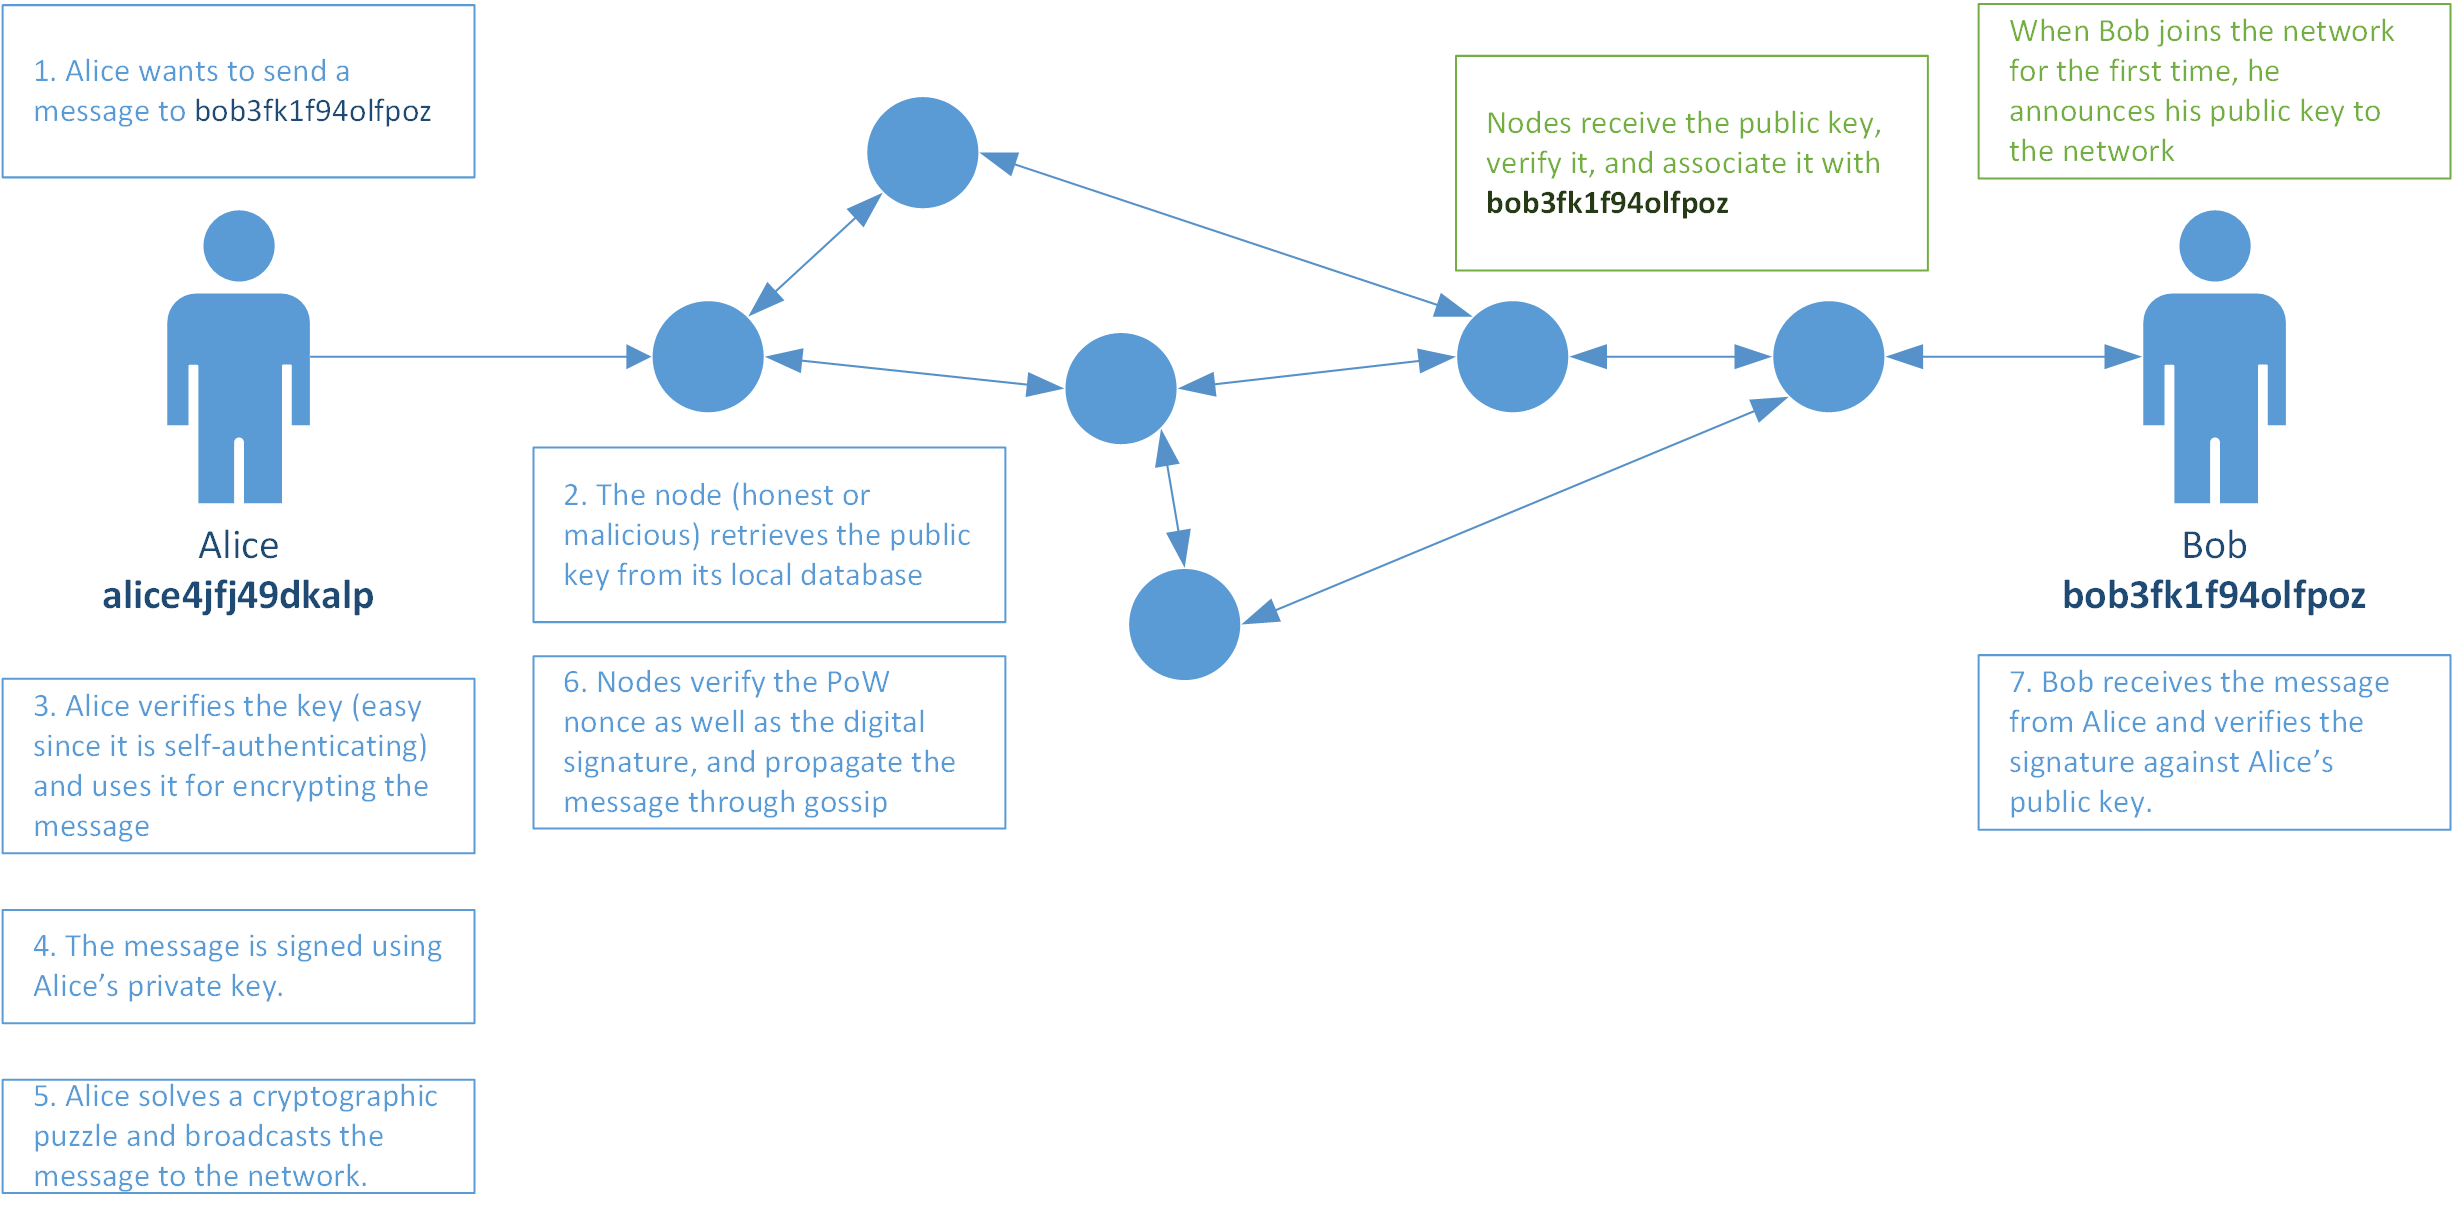
\includegraphics[width=\textwidth]{img/figure.png}
	\caption{Diagram that illustrates how users communicate.}
	\label{fig:figure}
\end{figure}

\section{Related work} % 0.5 pages
Relevant examples of end-to-end messaging systems are Telegram and Whatsapp. They are based on a public-key infrastructure, which means that there is a \emph{centralized} name directory that associates each user to a public key. Communications are realized by using standard cryptographic primitives: the sender encrypts the message with the recipient's public key and signs it with his/her private key. Then, the recipient can decrypt the message with his/her own private key and verify its authenticity. Our approach differs in the fact that there is no centralized name server: identities are derived from the public key, and as such are \emph{self-authenticating}.

This idea of self-authenticating names is not new. It has already been adopted by Tor (for hidden service names) and Bitcoin (for wallet addresses). A user that creates a Tor hidden service has to generate an RSA-1024 keypair that will be used for all encryption purposes. The \emph{.onion} address is computed by calculating the SHA-1 hash of the public key, and then by converting the first half to a Base32 string. As explained earlier, a name generated in such a way is random, but it is possible to brute-force a \emph{vanity name} of desired length (popular examples are \texttt{blockchainbdgpzk.onion}, \texttt{facebookcorewwwi.onion}, and \texttt{silkroad6ownowfk.onion}). Likewise, a Bitcoin wallet address (e.g. \texttt{14qENWZBHh4oXb7YU5hAAVGpEnZP8QWfWa}) is simply computed by hashing its public key and converting it to Base58. There is no actual record on the network that a given wallet has been created, unless money is sent to that address (which still does not guarantee that a wallet has actually been generated).

Finally, proof-of-work for spam prevention has been proposed for emails (\href{https://en.wikipedia.org/wiki/Hashcash}{Hashcash}), but its use is not widespread, mainly due to the lack of support by clients/servers and to the fact that it is not suitable for mailing lists. In our case, private messaging provides a more constrained scenario and could benefit from this mechanism.

%Finally, onion routing is one of the main features of Tor. Their implementation works by creating virtual circuits with TCP connections prior to initiating a communication. Packets are routed through 3 intermediary nodes before reaching the destination, and two-way communication is supported.
\section{Background} % 0.5 pages
We build on top of the first version of Peerster, which already implements the basic gossip primitives (rumormongering and anti-entropy). Instead of being sent directly to the recipients (which may be offline), messages are stored on the network. In principle, each node stores the full set of messages, but can also choose individual policies as long as they are compatible with the protocol. The storage of the full database provides the highest availability as well as \href{https://en.wikipedia.org/wiki/Plausible\_deniability}{plausible deniability}, that is, node maintainers cannot be held responsible for the content stored on the network. Moreover, in a \emph{private information retrieval} (PIR) context, this approach is theoretically secure because messages can be retrieved without revealing which item is being retrieved. As we will see in \Cref{sec:design}, the protocol allows for the implementation of \emph{lightweight nodes}, which trade off security for speed.

All cryptographic functionalities are implemented using the standard \emph{Crypto} library of Golang. Generally speaking, implementing one own's crypto primitives is a bad idea as it can lead to security vulnerabilities. This project makes massive use of hashing (SHA-256) and public-key cryptography using RSA. The details of the primitives are explained in detail in \Cref{sec:design}.

Finally, we use SQLite3 in combination with the driver \href{https://github.com/mattn/go-sqlite3}{go-sqlite3} for storing the local database in a persistent way. The local DB contains the public keys of all nodes, as well as all exchanged messages (public and private). 

\section{Design and architecture} % 0.75 pages
\label{sec:design}
The backbone of the network consists of the so-called \emph{full nodes} (analogous to Bitcoin full nodes), which exchange messages through a gossip mechanism, and store the entire database. The protocol allows for the existence of \emph{lightweight nodes} (i.e. clients), that can send or retrieve specific messages without contributing to the gossip. This design mostly focuses on full nodes, but the specification allows for some degree of flexibility. It is worth noting that, from a private information retrieval perspective, running a lightweight node reduces the amount of privacy because malicious nodes could see which messages are retrieved.

We now address the protocol, which is the most important part of the design. It should not be too restrictive (so as to enable functionality extensions and custom/optimized implementations), but at the same time should be secure by design (as eventual holes would break the consistency of the system). Our system is essentially based on two principles:
\begin{description}
	\item[No consensus:] consensus is useful because it directly ensures that all nodes agree on a certain set of items. It also provides strong guarantees about their order (in fact, the strongest: \emph{total order}). However, if no prior assumptions are made, it poses some serious drawbacks in terms of performance, scalability, and security.  Bitcoin (and other cryptocurrencies) implement a form of probabilistic consensus that improves some of these issues, but does not solve the problem entirely. Fortunately, we are implementing a private messaging service, which requires less guarantees (e.g. FIFO order instead of total order). Moreover, thanks to self-authenticating names, the system can be fully decentralized without requiring consensus.
	\item[Eventual consistency:] all nodes will eventually converge to the same state. This is ensured by gossip and by some security mechanisms that we describe below.
\end{description}

\subsection*{Name system}
In our reference implementation, each node is associated with \emph{one} identity. When the application is launched for the first time, a new identity is generated and identifies a certain node. However, the protocol does not strictly require this 1--1 association: a node could have multiple identities, or none (i.e. relay node).

An identity corresponds to an RSA-2048 keypair. The private key is used for signing and decrypting messages, while the public key is used for encrypting messages and identifying a user. Since the public key has a length of 256 bytes (+4 bytes for the exponent), it is not suitable as an ID that can be exchanged with other users. Therefore, similarly to Tor, we derive a \emph{display name} from the public key as follows: the public key is hashed using SHA-256; afterwards, we take the first 80 bits of the hash and we convert them to Base32. This produces a string of 16 alphanumeric characters. Being self-signing, names can be easily verified against the public key. This means that we do not need to store the full public key in every message, but, of course, the protocol should provide a way to exchange public keys (otherwise nodes would not be able to encrypt or verify messages).

\subsection*{Message format}
The protocol is entirely based on gossip messages, which follow a fixed layout. The SQLite table that stores the messages follows the same layout, i.e. gossip messages, if accepted, are stored in the database without any variation. Every message is tagged with an incremental ID \emph{relative to the sender}, which corresponds to implementing a vector clock. Therefore, a message is uniquely identified by its (Sender, ID) pair.\\
{
	\centering
	\resizebox{\textwidth}{!}{
	\begin{tabular}[c]{|l|l|l|l|l|l|l|}
		\hline
		Message ID & From & To & Content & Signature & PoW nonce\\
		\hline
		uint32 & string 16 chars & string 16 chars or empty & string or binary & binary or empty & binary 16 bytes\\
		\hline
	\end{tabular}}
	\vspace{2mm}
}\\
The table above shows how messages are structured. Every message must contain the \texttt{Message ID} (sequential number), \texttt{From}, and \texttt{Proof-of-Work Nonce} fields. The other fields depend on the specific message type:
\begin{itemize}
\item \textbf{Key announcement message:} this is a special message that is always identified by the \texttt{Message ID} = 0. The first message that a node sends when it joins the network is a key announcement message, and, as the name suggests, it contains the public key associated with a certain origin.\\
{
	\centering
	\resizebox{0.9\textwidth}{!}{
	\begin{tabular}[c]{|l|l|l|l|l|l|l|}
		\hline
		Message ID & From & To & Content & Signature & PoW nonce\\
		\hline
		0 & \texttt{alice4jfj49dkalp} & -- & Serialized public key & -- & Binary data\\
		\hline	
	\end{tabular}}
	\vspace{2mm}
}\\
The \texttt{To} field is absent because this is a public message intended for everyone. The \texttt{Signature} is absent because it would be redundant, as names are self-signing. In our case, the serialized public key has a length of 2048 bits = 256 bytes, plus 4 bytes for the exponent (uint32 little endian).

\item \textbf{Public message:} this is a message sent to the public chat room. Messages are not encrypted as they should be visible to everyone, but are signed in order to confirm the identity of the sender.\\
{
	\centering
	\resizebox{0.9\textwidth}{!}{
	\begin{tabular}[c]{|l|l|l|l|l|l|l|}
		\hline
		Message ID & From & To & Content & Signature & PoW nonce\\
		\hline
		1234 & \texttt{alice4jfj49dkalp} & -- & Hello! & Binary data (256 bytes) & Binary data\\
		\hline	
	\end{tabular}}
	\vspace{2mm}
}\\
\item \textbf{Private message:} these messages are identified by the presence of the \texttt{To} field, and require the content to be encrypted.\\
{
	\centering
	\resizebox{0.9\textwidth}{!}{
	\begin{tabular}[c]{|l|l|l|l|l|l|l|}
		\hline
		Message ID & From & To & Content & Signature & PoW nonce\\
		\hline
		1234 & \texttt{alice4jfj49dkalp} & \texttt{bob3fk1f94olfpoz} & Binary data & Binary data & Binary data\\
		\hline	
	\end{tabular}}
	\vspace{2mm}
}\\
Since the message should be visible to both the sender and the recipient, its content is encrypted twice (separately), respectively with the private key of the sender and with the private key of the recipient. The encryption uses RSA with an \href{https://en.wikipedia.org/wiki/Optimal\_asymmetric\_encryption\_padding}{OAEP} padding scheme, which guarantees that the same cleartext is not encrypted into the same ciphertext, and prevents information leakage from the original length of the message. The OAEP is parameterized with a SHA-256 hash function. All messages encrypted in such a way have a fixed length of 256 bytes (i.e. the length of the public key), and the maximum length of a message is 190 bytes.
The format of the \texttt{Content} field starts with a \texttt{uint16} (little endian) that encodes the length of the first ciphertext (i.e. the message encrypted with the private key of the sender). Then, we concatenate the sender ciphertext and the recipient ciphertext. In other words, the binary data is represented as \texttt{len1 | cipher1 | cipher2}. In our case, this field has a fixed length of 2+256+256=514 bytes, but in the more general case it can accommodate for different key lengths.
\end{itemize}

It can be observed that there is no physical timestamp (time field) that describes when a message is sent. The reason is that timestamping in a decentralized and adversarial setting requires consensus/total order. Instead, we rely on the causal order provided by vector clocks.

\subsection*{Signature scheme}
Messages are signed using \href{https://en.wikipedia.org/wiki/Probabilistic\_signature\_scheme}{RSA-PSS}, which is provably secure. The signature is calculated on the SHA-256 hash of all fields except the proof-of-work nonce (which must be computed as final step before sending the message). The verification of a message, of course, follows the same steps.

\subsection*{Proof-of-work scheme}
The \texttt{proof-of-work nonce} field of a \emph{new} message must be filled prior to broadcasting it for the first time. Every message, regardless of its type, must contain a valid nonce in order to be accepted by other nodes.
A message is associated with a unique SHA-256 hash, which is not transmitted along with its content, but can be easily computed and verified. More specifically, the hash is computed on all fields \emph{including} the nonce, which has a length of 16 bytes in our reference implementation, and can contain any value.

As a spam prevention mechanism, the hash of a message must start with a certain number of leading zeros, which is specified in the configuration of the node. Every zero doubles the computational cost associated with producing a valid hash. The reference implementation starts with a nonce of zero, and increments it until the hash of the message reaches the desired target. Enforcing this mechanism to all messages (including key announcements) ensures that identities are hard to create, in addition to text messages.

It is important to understand that the nonce must be computed only by the original sender of the message, and not by other nodes on the network. Upon the reception of a message, nodes verify the hash and store the message along with its nonce in the local database, so that they need not recompute it. Likewise, if the message is rebroadcast through gossip, the original nonce is included in the packet.

\subsection*{Exchange protocol}
The protocol for sending a message works as follows: Alice (e.g. \texttt{alice4jfj49dkalp}) wants to send a message to Bob (e.g. \texttt{bob3fk1f94olfpoz}). The message is encrypted with her own public key (because she must be able to see her own messages), as well as Bob's public key, which can be easily retrieved by knowing Bob's display name and getting his key announcement message, i.e. the very first one with ID = 0. If the announcement message cannot be found, either Bob does not exist, or his key has not fully propagated over the network. As the key announcement is sent right after generating a new identity, the latter case is unlikely. Additionally, Alice signs the message with her private key. Finally, she computes the proof-of-work nonce such that the SHA-256 hash of the message starts with the target number of leading zeros, and starts the rumormongering process to distribute the message.

Nodes that receive a gossip message run a series of verification steps prior to accepting it:
\begin{enumerate}
\item The message is first checked for correctness (correct deserialization, layout, field lengths and content).
\item Its hash is computed and verified for proof of work.
\item If it is a regular private/public message, the digital signature is verified. Likewise, if it is a key announcement message, the name is verified against the public key.
\item If all tests pass, the message is accepted into the application logic, otherwise it is dropped silently.
\end{enumerate}

An accepted message is stored in the local database as-is, if not already so. If applicable (that is, if the message is unseen), the message is redistributed through rumormongering.

We must also define a rule for resolving conflicts. In a possible attack scenario, imagine that a sender sends different messages with the same sequence ID to different peers. This would create an inconsistency in the network, because some nodes would store one version of the message, whereas others would store another one. One way to guarantee the \emph{eventual consistency} property without requiring consensus is to define a \emph{lexicographical preference} on the messages. Our rule is: the message with the lowest hash is preferred. In other words, if a node receives a message with an (origin, ID) pair that is already stored in the database, the old message is replaced if the hash of the new message is lower than the hash of the old message. Moreover, this mechanism allows the proof-of-work difficulty to increase over time (as users can recompute nonces of existing messages). On the other hand, this approach has the side effect of allowing users to modify their own messages (albeit in a detectable way and with increasing difficulty). Whether this is acceptable or not can be argued, but it is worth noting that in a distributed system there is always some kind of trade-off between guarantees and performance.

\section{Evaluation} % 0.5 pages
\subsection*{Weaknesses}
The first part of the evaluation was purely theoretical and was aimed at finding strong points and weaknesses in the protocol, from a security/privacy/performance viewpoint. Many design choices represent a trade-off between security and performance, and it is important to identify eventual side effects associated with them.

As stated earlier, it is impossible to devise a protocol that provides strong guarantees in all scenarios, as some form of compromise is always necessary. In the previous section we reported such an example (conflicting messages from the same sender, which are resolved by taking the one with the lowest hash).

A weakness of our protocol is that it does not guarantee metadata anonymity: the sender and recipient of a message are publicly visible, and in theory it could be possible to associate some users with certain activities. On a positive note, identities are anonymous, unless users decide to reveal them deliberately. Moreover, nothing prevents users to create new identities to communicate with different people. In fact, just like Bitcoin addresses, this practice is encouraged. An alternative design choice would have been to put the sender inside the encrypted content, thus guaranteeing \emph{sender anonymity}. However, this choice opens to some attacks: anyone could send forged messages, which intermediate nodes would not be able to verify. Only the recipient would be able to know the original sender and verify the signature, but, in principle, anyone could congest his/her message box with corrupted messages. In our scenario, it would also be possible to tamper with the vector clocks and replace messages.

As for the performance of the system, vector clocks represent a problem because their size grows linearly with the number of identities. There are some techniques for mitigating this issue, like pruning. Another approach would be to use a different message synchronization algorithm for the anti-entropy functionality, perhaps based on Merkle trees, as some popular NoSQL DBMSs like \href{https://wiki.apache.org/cassandra/AntiEntropy}{Dynamo or Cassandra do}. However, this was not implemented as it is out of the scope of this project.

Another potential weakness is that, since there is no consensus mechanism, nodes must cooperatively agree on the proof-of-work difficulty. Doing this at the beginning is easy, as the optimal value could be defined in the protocol. However, increasing the difficulty over time is trickier. One option is to let nodes decide for themselves: they will not probably agree on the set of messages, but the network would nonetheless function correctly.


\subsection*{Correctness}
The second part of the evaluation was targeted at verifying that all specifications were met without introducing bugs or security holes in the protocol, through a combination of code inspection and manual tests. In particular, the tests were devised so as to test each feature individually before moving to more complex cases: first, we tested the basic gossip functionalities, then we tested the public messaging system (along with the signature verification); finally, we tested the private messaging system. Furthermore, packets were inspected using Wireshark and the database was manually checked using an SQLite3 database explorer.

The full system was tested on a simulated network topology, and on a local network. We did not find considerable bottlenecks in the software, especially because Go is a compiled language. The limiting factor is represented by the network and disk I/O for reading from/writing to the local database. The proof-of-work mechanism helps because it provides a natural way of limiting the rate of messages. By setting the average computation time in second and knowing the number of nodes, it is possible to estimate an upper bound of the bandwidth requirement.



\end{document}